\chapter{Quantum Distribution Key (QDK)}
\section{Introduzione}
\begin{itemize}
	\item Il protocollo QDK è un protocollo alternativo a Diffie-Hellman per lo scambio delle chiavi.
	\item Permette di scambiare lunghe chiavi da utilizzarsi con one-time pad.
	\item Inoltre è già utilizzato in quanto non necessita dell'utilizzo di computer quantistici e se in futuro la tecnologia quantistica dovesse evolversi comunque questo protocollo sarebbe quantistico-resistente oltre che resistente al collasso della classe NP.
	
	Questo protocollo inoltre permette di accertare una eventuale intrusione, eventualmente si butta via la chiave, proprio per questo motivo non si può usare per scambiare messaggi.
\end{itemize}
\paragraph{NB} Esiste poi la crittografia post-quantistica che si occupa di cercare sistemi a chiave pubblica inattaccabili anche da macchine quantistiche. Ci si basa su problemi NP-completi che si sanno essere difficili anche con una eventuale supremazia quantistica.

\subsection{Principi della meccanica quantistica}
Sfruttiamo i seguenti principi della meccanica quantistica.
\begin{itemize}
    \item \textbf{Sovrapposizione degli stati}
    
    Un sistema quantistico si può trovare in più di uno stato allo stesso tempo. Matematicamente si intende una combinazione lineare dei possibili stati (i coefficienti sono numeri complessi). Il quadrato del modulo è la probabilità di individuare un particolare stato, quando effettuiamo una misurazione.
    
    \item \textbf{Decoerenza}.
    
    Quando si effettua una misurazione il sistema si \emph{perturba} quindi collassa solo in uno degli stati che prima erano sovrapposti. Si lascia quindi una traccia all'atto della misurazione, la usiamo per controllare circa eventuali intromissioni nella trasmissione
    
    \item \textbf{No-cloning}.
    
    Impossibilità di fare una copia di un sistema quantistico.
    Per copiare bisogna misurare, ma misurare significa modificare il sistema e quindi lasciare una traccia.
    \[\boxed{\text{No osservazione, no copia}}\]
    
    \item \textbf{Entanglement}.
    
    La possibilità che due sistemi creati con una correlazione tra loro continuino a mantenere la correlazione anche se portati a grandi distanze l'uno dall'altro (al contrario del principio di località della fisica classica). Quindi una misura eseguita su uno dei due influenza anche lo stato dell'altro seppur a larghissima distanza.
    
    \textbf{Esempio del fratello del prof. Luccio}: \emph{Il vostro partner va in Australia, se il vostro partner vi tradisce in quello stesso momento diventate cornuti (pur essendo a migliaia di chilometri di distanza)}.
\end{itemize}

\section{Protocollo BB84}
Nasce nel 1984 da Bennet e Brassard. Si fa tramite lo scambio di \emph{fotoni polarizzati} (particella elementare che costituisce la luce corpuscolare). Ogni fotone ha varie proprietà:
\begin{itemize}
	\item non ha massa;
	\item si muove alla velocità della luce;
	\item ha una sua \emph{polarizzazione} (piano di oscillazione del suo campo elettrico).
\end{itemize} 
Gli stati di polarizzazione da noi considerati sono quattro, che per comodità raggruppiamo in due \emph{basi di polarizzazione}.
\begin{center}
    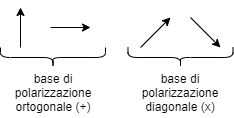
\includegraphics[width=150px]{images/QDK_1.png}
\end{center}
La direzione di polarizzazione può essere qualsiasi quindi scegliamo una base per rappresentarla (come se fosse un vettore).
In ognuno di questi stati codifichiamo un bit:
\begin{multicols}{2}
\begin{itemize}
    \item \textbf{verticale}: 0
    \item \textbf{orizzontale} : 1
    \item \textbf{+45°}: 0
    \item \textbf{-45°}: 1
\end{itemize}
\end{multicols}
\noindent Le scelte sono arbitrarie, stabilite dagli interlocutori: sanno quale base è stata adottata e compiono misurazioni secondo la base adottata. Se non si conosce quale base è stata usato non possiamo effettuare misurazioni corrette e certe ma solo probabilistiche: nel protocollo ci baseremo proprio su questa probabilità! La misura è completamente casuale perchè a seguito di una misurazione andiamo ad alterare il sistema, dunque perdiamo le informazioni precedenti.
\subsection{Premessa: struttura generale dell'hardware}
\begin{center}
    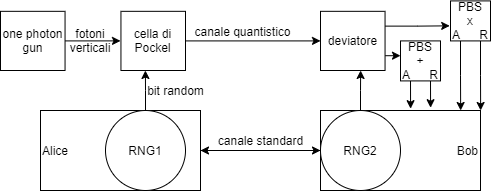
\includegraphics[width=300px]{images/QDK_2.png}
\end{center}
Ci si muove su due canali:
\begin{itemize}
	\item uno quantistico (fibra ottica), 
	\item uno standard (Alice e Bob devono comunicarsi le basi che hanno utilizzato per misurare, vedremo bene più avanti).
\end{itemize}
\paragraph{Lato Alice}  Supponiamo che Alice voglia trasmettere un messaggio a Bob.
\begin{itemize}
    \item \textbf{One Photon Gun}: emette singoli fotoni, tutti con polarizzazione verticale.
    \item \textbf{Cella di Pockel}: impone una certa polarizzazione. Questa è scelta da un \emph{Random Number Generator}, cioè Alice sceglie casualmente la polarizzazione del fotone.
\end{itemize}
\paragraph{Lato Bob} Bob riceve i fotoni, ma non sa cosa vuole trasmettere Alice. Non ha presente neanche la base: segue che per prima cosa dovrà scegliere come misurare il fotone, lo fa in modo casuale attraverso un \emph{Random Number Generator}.
\begin{itemize}
	\item \textbf{SW}: \textit{deviatore}, che si comporta in base al valore scelto da RNG2. In base al valore scelto cambia lo strumento con cui misuriamo il fotone.
    \item \textbf{PBS} (\emph{Beam splitter polarizzante}): ci da la corretta polarizzazione del fotone \textbf{se e solo se} la base di generazione e la base di misurazione sono le stesse utilizzate da Alice al momento dell'invio del fotone.
\end{itemize}
\subsubsection{\emph{Beam Splitter Polarizzante} (PBS)}
Il Beam Splitter polarizzante presenta un suo asse di polarizzazione $S$, in contrasto con la polarizzazione $F$ del fotone arrivato, mentre $\theta$ è l'angolo tra le due direzioni di polarizzazione. Misura il fotone tramite la deviazione verso una delle due uscite: 
\begin{itemize}
	\item A (assorbimento)
	\item R (riflessione)
\end{itemize}
La polarizzazione uscente non è quella del fotone in ingresso, ma una delle due polarizzazioni del PBS: $S$ o $S$ ortogonale. Da cosa dipende l'uscita? Dall'angolo $\theta$. Affermiamo che il fotone:
\begin{itemize}
    \item esce da A (polarizzazione $S$) con probabilità $\cos^2 \theta$
    \item esce da R (polarizzazione $S$ ortogonale) con probabilità $\sin^2 \theta$
\end{itemize}
\paragraph{Esempi in cui la polarizzazione è mantenuta} Può succedere che la polarizzazione uscente sia la stessa del fotone entrante. Sia $F$, ribadiamo, la polarizzazione del fotone entrante.
\begin{itemize}
    \item Se $\theta = 0$ abbiamo $F=S$, il fotone ha la stessa polarizzazione dello strumento. Le probabilità sono: 
    \begin{multicols}{2}
    \begin{itemize}
    	\item $\sin^2 \theta=0$ che esca da $R$;
    	\item $\cos^2\theta=1$ che esca da $A$.
    \end{itemize}
	\end{multicols}
	Il fotone uscirà sicuramente da $A$, con polarizzazione $S$.
    \item Se $\theta = 90$ allora $F \perp S$. Abbiamo come probabilità: 
    \begin{multicols}{2}
    \begin{itemize}
    	\item $\sin^2 \theta = 1$ che esca da $R$;
    	\item $\cos^2 \theta = 0$ che esca da $A$.
    \end{itemize}
\end{multicols} Il fotone uscirà sicuramente da $R$ e avrà come polarizzazione $S$ ortogonale. Anche in questo caso si conserva.
\end{itemize}
\paragraph{Distruzione dello stato precedente} Se $\theta = \pm45^{\circ}$ le basi di misurazione e di generazione sono diverse. Abbiamo come probabilità:
$$\cos^2\theta = \sin^2\theta = \frac{1}{2}$$
Il fotone ha pari probabilità di uscire da A o da R. La lettura attraverso il PBS potrebbe quindi distruggere lo stato quantistico precedente. Ricapitolando
\begin{center}
    \begin{tabular}{c|c|c|c|c}
        & 0 $\uparrow$ & 0 $\nearrow$ & 1 $\rightarrow$ & 1 $\searrow$ \\
        \hline
        + & $\uparrow$ & $\uparrow \rightarrow$ & $\rightarrow$ & $\uparrow \rightarrow$  \\
        x & $\nearrow \searrow$ & $\nearrow$ & $\nearrow \searrow$ & $\searrow$
    \end{tabular}
\end{center}
Le colonne indicano \textbf{bit e fotone inviato da Alice}, le righe \textbf{le basi di Bob}. Si ribadisce quanto già detto: se la base coincide si ottiene lo stesso stato, se la base non coincide allora lo stato precedente viene distrutto (i possibili stati sono equiprobabili). 
\subsection{Step del protocollo} 
Andiamo dunque al protocollo:
\begin{enumerate}
    \item Alice invia una sequenza $S_A$ sul canale quantistico.\\ Si segna le basi usate per generare i fotoni.
    \item Bob interpreta $S_A$ con le basi scelte casualmente.\\ Si segna quali basi ha usato per effettuare le misurazioni dei fotoni.
    \item Bob comunica ad Alice le sue basi \textbf{\underline{sul canale standard}}
    \item Alice risponde dicendo quali basi sono comuni alle sue.\\Dove le basi sono concordi si prendono i bit, dove le basi sono discordi si buttano.
\end{enumerate}
Si ha circa il 50\% di match. Alice e Bob, a seguito del confronto e in assenza di interferenze di Eve, possiedono $S_A' = S_B'$ sottosequenze identiche formate dai bit codificati dal mittente e decodificati dal destinatario con basi comuni:
$$ \mid S_A' \mid = \mid S_B' \mid = \frac{\mid S_A \mid}{2} $$
\paragraph{Variante al protocollo} Esiste un altro algoritmo quantistico di scambio di chiavi che si basa sull'entanglement: se i due estremi misurano con la stessa base fotoni correlati sono correlati anche i loro risultati quindi A e B misurano chiavi complementari.

\subsection{Esempio}
Consideriamo il seguente esempio, dove Alice trasmette una sequenza a Bob
\begin{center}
    \begin{tabular}{c|c c c c c c c c }
        $S_A$: & 1 & 0 & 1 & 1 & 1 & 0 & 0 & ...  \\
        Base adottata da alice: & + & x & + & x & x & + & x & ... \\
        Fotoni inviati da Alice: & $\rightarrow$ & $\nearrow$ & $\rightarrow$ & $\searrow$ & $\searrow$ & $\uparrow$ & $\nearrow$ & ...  \\
    
        & & & & & & & &  \\

        Base adottata da Bob: & + & x & + & + & + & x & x & ...  \\
        Lettura di Bob: & $\rightarrow$ & $\nearrow$ & $\rightarrow$ & $\uparrow$ 50\% & $\rightarrow$ 50\% & $\searrow$ 50\% & $\nearrow$ & ... \\
        $S_B$: & 1 & 0 & 1 & 0 & 1 & 1 & 0 & ...  \\
    \end{tabular}
\end{center}
Le basi concordi sono 1, 2, 3, 7 che portano alla sequenza:
$$ S_A' = S_B' = 1010 $$
Le riflessioni sarebbero già finite in assenza di crittoanalisti...

\subsection{Presenza del crittoanalista ed errori sperimentali}
La questione fondamentale è che la presenza del crittoanalista altera lo stato di polarizzazione dei fotoni (ricordare la proprietà della \emph{decoerenza}). 
\begin{itemize}
	\item Se c'è un crittoanalista esso si troverà nella stessa situazione di Bob, quindi deve scegliere le sue basi.
	\item Le basi scelte da Eve saranno indipendenti sia da quelle di Alice che da quelle di Bob. Se la base scelta da Bob coincide con quella di Alice allora non cambia nulla, se non coincide altera irreparabilmente il fotone!
	\item \textbf{Soluzione}. Alice e Bob fanno una verifica sacrificando un pezzo di $S_A'$ e $S_B'$:
	si scambia una porzione delle chiavi comuni in posizioni prestabilite comunicandole sul canale standard. A quel punto:
	\begin{itemize}
		\item se le due sequenze sono diverse la comunicazione viene interrotta;
		\item altrimenti usano la porzione rimanente come chiave o per costruire la chiave.
	\end{itemize}	
\end{itemize}
Riprendiamo l'esempio precedente e vediamo cosa succede con Eve nel mezzo:
\begin{center}
    \begin{tabular}{c|c c c c c c c c}
        $S_A$: & 1 & 0 & 1 & 1 & 1 & 0 & 0 & ... \\
        Base adottata da Alice: & + & x & + & x & x & + & x & ... \\
        Fotoni inviati da Alice: & $\rightarrow$ & $\nearrow$ & $\rightarrow$ & $\searrow$ & $\searrow$ & $\uparrow$ & $\nearrow$ & ... \\
    
        & & & & & & & & \\

        Base adottata da Eve: & + & + & + & x & + & x & + & ... \\
        Lettura di Eve: & $\rightarrow$ & $\rightarrow$ 50\% & $\rightarrow$ & $\searrow$ & $\uparrow$ 50\% & $\nearrow$ 50\% & $\rightarrow$ 50\% & ... \\
        $S_E$: & 1 & 1 & 1 & 1 & 0 & 0 & 1 & ... \\

        & & & & & & & & \\

        Base adottata da Bob: & + & x & + & + & + & x & x & ... \\
        Lettura di Bob: & $\rightarrow$ & $\searrow$ 50\% & $\rightarrow$ & $\uparrow$ 50\% & $\uparrow$ & $\nearrow$ & $\searrow$ 50\% & ... \\
        $S_B$: & 1 & 1 & 1 & 0 & 0 & 0 & 1 & ... \\
    \end{tabular}
\end{center}
\noindent Prendiamo i valori con basi concorde:
$$ S_A' = 1010 \neq  1111 =S_B' $$
\begin{itemize}
	\item Supponiamo quindi che si sacrifichi il secondo bit: $0 \neq 1$ e quindi ci si accorge di una intrusione.
	\item I bit non perturbati sono quelli per cui le 3 basi coincidono: $\frac{1}{4}$ delle volte. Quindi se Eve interviene: circa la metà di $S_A'/S_B'$ sarà differente.
	\item La verifica dell'intrusione è quindi importantissima, permette di sapere di eventuali intrusioni e quindi evitare di perdere informazioni.
\end{itemize}
Si osservi che le variazioni nello stato di polarizzazione non dipendono solo dall'intrusione di Eve: possiamo avere errori generici in fase di trasmissione dei fotoni, delle letture, ecc...
\begin{itemize} 
	\item Si stabilisce un \textbf{\emph{quantum bit error rate}} (QBER): una percentuale prevedibile di bit errati (dovuti a errori dell'apparato sperimentale).
	\item Si confrontano $S_A'$ e $S_B'$:
	\begin{itemize}
		\item se il numero di errore è $>$ QBER allora c'è stata una intromissione (e interrompiamo la comunicazione);
		\item altrimenti sono solo errori sperimentali e si correggono tramite correttori di errori.
	\end{itemize}	
	\item Eve potrebbe intercettare pochi fotoni e quindi farsi passare per errori dell'apparato pur conoscendo alcuni bit della chiave. Proprio per questo motivo anziché usare la sequenza scambiata si usa farne l'hash ed usare quello come chiave, in questo modo se cambiano anche solo pochi bit l'hash cambia enormemente.
	
	\item Le comunicazioni su canale standard possono anche essere in chiaro, è bene tuttavia che siano autenticate, magari tramite MAC (simmetrico con chiave scambiata in anticipo).
\end{itemize}
